%%%%%%%%%%%%%%%%%%%%%%%%%%%%%%%%%%%%%%%%%%%%%%%%%%%%%%%%%%%%%%%%%%%%%%%%%%%%%%%%%%%
% 			Facultad de Ciencias, UAEM.							Agosto de 2013
% 
%	Alumno: 				Emanuel García Perez
%	Asginatura:				Computación y Sociedad
%	Proyecto:				Exposición
%	Tema:					"Censura en Internet // OpenNet Initiative"
%
%%%%%%%%%%%%%%%%%%%%%%%%%%%%%%%%%%%%%%%%%%%%%%%%%%%%%%%%%%%%%%%%%%%%%%%%%%%%%%%%%%%


\documentclass{beamer}

\usepackage[spanish,activeacute]{babel}
\usepackage[latin1]{inputenc}
\usepackage{beamerthemeshadow}
\usepackage{graphicx}

\title{\textbf{Censura en Internet // OpenNet Initiative}}
\author{Emanuel Garc\'ia P\'erez}
\date{\today}

\begin{document}

\frame[allowframebreaks]{\titlepage}
\section[Contenidos]{}
\frame{
\transdissolve[duration=0.2]
\tableofcontents
}


\section{Censura}
\frame
{
\transdissolve[duration=0.2]
\frametitle{?`Qu\'e es la Censura?}
Practica que implica la supresi\'on de contenido de un material de comunicaci\'on por razones ideol\'ogicas, morales o pol\'iticas; cuando cierto contenido es considerado ofensivo, da\~nino, inconveniente o innecesario suele ser censurado por un medio de comunicaci\'on, el gobierno o cualquier otro organismo que as\'i lo determine.
}

\subsection{Justificaciones}
\frame{
\transdissolve[duration=0.2]
\frametitle{Censura Moral}
\begin{figure}
  \centering
    
\includegraphics[width=0.4\textwidth]{cens_1.jpg}
  \label{fig:ejemplo}
\end{figure}
}

\frame{
\transdissolve[duration=0.2]
\frametitle{Censura Militar}
\begin{figure}
  \centering
    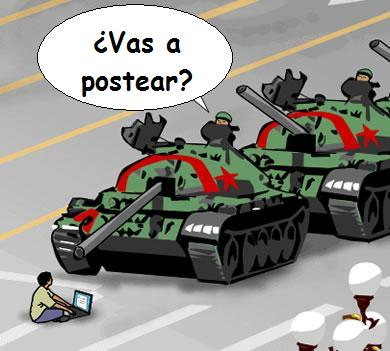
\includegraphics[width=0.6\textwidth]{cens_post.jpg}
  \label{fig:ejemplo}
\end{figure}
}

\frame{
\transdissolve[duration=0.2]
\frametitle{Censura Pol\'itica}
\begin{figure}
  \centering
    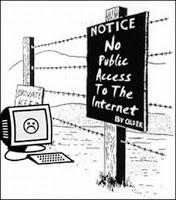
\includegraphics[width=0.5\textwidth]{cens_int.jpg}
  \label{fig:ejemplo}
\end{figure}
}

\frame{
\transdissolve[duration=0.2]
\frametitle{Censura Religiosa}
\begin{figure}
  \centering
    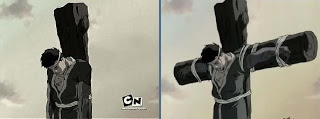
\includegraphics[width=0.7\textwidth]{cens_4.jpg}
  \label{fig:ejemplo}
\end{figure}
}

\frame{
\transdissolve[duration=0.2]
\frametitle{Censura Corporativa}
\begin{figure}
  \centering
    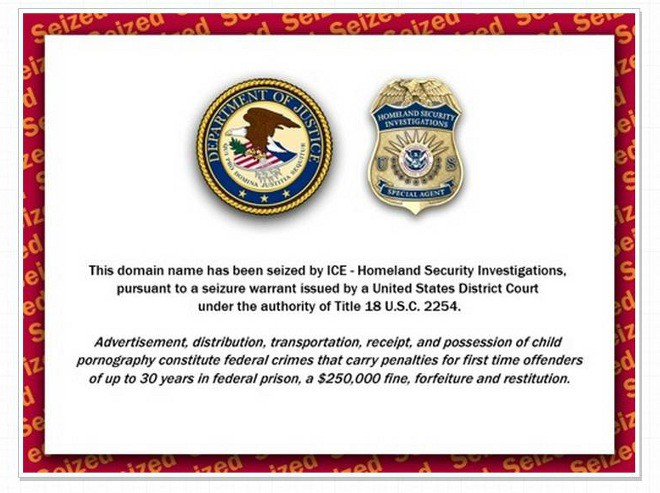
\includegraphics[width=0.7\textwidth]{bloq_int.jpg}
  \label{fig:ejemplo}
\end{figure}
}


\section{Censura en Internet}
\frame
{
\transdissolve[duration=0.2]
\frametitle{?`Qu\'e es la Censura en Internet?}
Todas las normas, t\'ecnicas y m\'etodos que utilizan ciertos grupos y organismos para controlar, manipular y/o suprimir determinados contenidos en Internet.
}

\subsection{Principales Contextos de Censura}
\frame
{
\transdissolve[duration=0.2]
\frametitle{Informaci\'on y Contenidos.}
\begin{enumerate}
\item Noticias y Opiniones.
\item Contenidos Religiosos.
\item Contenidos Eroticos/Sexuales.
\item Delincuencia.
\item Difusi\'on de Material Il\'icito.
\item Contenido Multimedia.
\end{enumerate}
}

\section{Casos Documentados}
\subsection{Art\'iculo - CEPREDE}
\frame
{
\transdissolve[duration=0.2]
\frametitle{La frontera entre la libertad de expresi\'on y la censura en Internet}
\begin{itemize}
\item En el mundo existe cerca de un 13\% de internautas que se encuentra sometido a una censura que les impide expresarse libremente en la red.
\item El grado de penetraci\'on de Internet en Cuba es de los m\'as bajos del mundo y est\'a aparejado con un grado de censura muy alto.
\item Con un nivel elevadisimo de censura pero con un mayor volumen de usuarios de Internet aparece China.
\end{itemize}
}

\subsection{Art\'iculo - Universidad SEK de Segovia}
\frame
{
\transdissolve[duration=0.2]
\frametitle{Censura en la Red: Restricciones a la Libertad de Expresi\'on en Internet}
Formas de Censura en la Red.
\begin{itemize}
\item Prohibici\'on de acceso a Internet(Afganistan, Corea del Norte).
\item Control de acceso a la Red mediado por la expedici\'on de autorizaciones exclusivas a personas de confianza(Cuba).
\item Monitorizaci\'on de Contenidos(China, Rusia, India, etc).
\item Filtrado de contenidos y bloqueo de sites(Arabia Saud\'ita).
\item Otras formas de censura(Campa\~nas de propaganda, Leyes de regulaci\'on, Software de filtrado, Redes de Espionaje, etc).
\end{itemize}
}

\end{document}
